\subsection{Method definition}

The basic idea of the \zm~method is to use a ``fake-rate'' method~\cite{fakeLeptonNote1,fakeLeptonNote2} based on \met.

Given a background process $B$ and a particular cut $c$ in the analysis suppressing $B$, a fake-rate method
estimates the yield of $B$ passing $c$ as the number of $B$ events failing $c$  
times a pass-to-fail ratio $R_{p-f}$
\begin{equation}
N_B\left(\mathrm{pass}\right)=N_B\left(\mathrm{fail}\right) \cdot R_{p-f}~,
\end{equation}
where $R_{pf}$ has to measured in an independent control sample 
reproducing with good accuracy the behavior of $B$ with respect to $c$.

Assuming that both in photon and \dyll~ events the sources of \met are the hadronic recoil against and pile-up effects, 
the \zm~method uses the \gjets~ sample to model the \met distribution in \dyll~events.
It defines a pass-to-fail ratio (\zm$\equiv$$R_{p-f}$) in bins of $N_{jets}$ and $p_{T}\left(\gamma\right)$:
\begin{equation}
\zeta\left(N_{jets},p_{T}\left(\gamma\right)\right)=\frac{N\left(N_{jets},p_{T}\left(\gamma\right), \met>\mwp\right)}{N\left(N_{jets},p_{T}\left(\gamma\right),\met<\mwp\right)}
\end{equation}
where $\mwp$ represents the working point chosen for the final \met~cut in the analyis.

In the same flavor dilepton sample, events passing the final analysis
selection but with $\met<\mwp$ are selected and \zm~is used to extrapolate to the signal region:
\begin{equation}
N_{\dyll}\left(\met>\mwp,N_{jets},p_{T}\left(\dil\right)\right)= \zeta\left(N_{jets},p_{T}\left(\dil\right)\right) \cdot N_{\dyll}\left(\met<\mwp,N_{jets},p_{T}\left(\dil\right)\right)
\end{equation}
where, in data, $N_{\dyll}\left(\met<\mwp\right)$ is computed subtracting opposite flavor and \V\Z~ events.

A corollary of the method is that shapes can be obtained from data by filling the histogram with \dyll~ events in the \met$<$\mwp~region 
with weight \zm~ (the same procedure is already used in 2011 analysis for the \Wjets~ background\cite{ref:shapenote}).

\subsection{The \hww~case}

In the \hww~analysis we consider events with dilepton $p_T$$>$45 \GeVc~and $\mathrm{min}$-$\mathrm{pmet}$$>$20 \GeV~ as a baseline common to same and opposite flavor final state~\cite{ref:hwwsmurfs};
$\mathrm{min}$-$\mathrm{pmet}$ is defined as:
\begin{equation}
\text{min-pmet} = \text{min(proj-pfMet,proj-trackMet)} ,
\end{equation}
where ``pfMet'' is the \met~reconstructed with the particle flow algorithm, ``trackMet'' is the \met~ constructed from charged particles consistent 
with originating from the primary vertex.
The ``proj-met'' variable (where met is either pfMet or trackMet) is defined as:
\begin{equation}
\text{proj-met} = 
\begin{cases} \met & \text{if $\Delta\phi_{min}>\frac{\pi}{2}$,}
\\
\met\sin(\Delta\phi_{min}) & \text{if $\Delta\phi_{min}<\frac{\pi}{2}$}
\end{cases}
\end{equation}
\begin{equation}
\text{with } \Delta\phi_{min} =  min(\Delta\phi(\ell_1,\met),\Delta\phi(\ell_2,\met))\\
\end{equation}
where $\Delta\phi(\ell_i,\met)$ is the angle between \met\ and lepton $i$ in the transverse plane;
the main purpose for using ``proj-met'' is to reduce the impact of lepton mismeasurement and, secondarily, to further suppress the contribution from \dytt.
The final \met~ selection in the same flavor dilepton final state requires min-pmet$>$(37+nvtx/2) \GeV. 

In the photon sample this selection is reproduced by cutting on min-met=$\mathrm{min(pfMet,trackMet)}$ and photon $p_T$.
In photon events, ``proj-met'' variables cannot be defined because is not possible to project on lepton directions, so the \zm~ method will not 
predict the contribution from fake \met~due to lepton mismesurement. 
However, as it shown in Figures \ref{fig:met_0j}-\ref{fig:met_1j}, despite the slightly different definiton, the photon sample reproduces with 
good precision the \met in the \dyll~sample.

Is summary, we use the following definitions:
\begin{itemize}
\item dilepton sample pass region: min-pmet$>$(37+nvtx/2) \GeV, dilepton $p_T$$>$45 \GeVc
\item dilepton sample fail region: 20$<$min-pmet$<$(37+nvtx/2) \GeV, dilepton $p_T$$>$45 \GeVc
\item photon sample pass region: min-met$>$(37+nvtx/2) \GeV, photon $p_T$$>$45 \GeVc
\item photon sample fail region: 20$<$min-met$<$(37+nvtx/2) \GeV, photon $p_T$$>$45 \GeVc
\end{itemize}

%%%%%%%%
\begin{figure}[!hbtp]
\begin{center}
\subfigure[proj-pfMet in \dyll~ sample]{\label{subfig:pmet_0j}
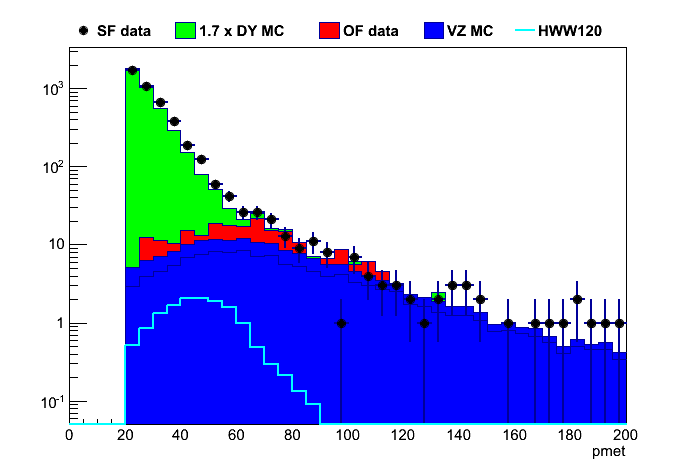
\includegraphics[width=.4\textwidth]{figures/pmet_0j.png}}
\subfigure[pfMet in \gjets~ sample]{\label{subfig:met_0j}
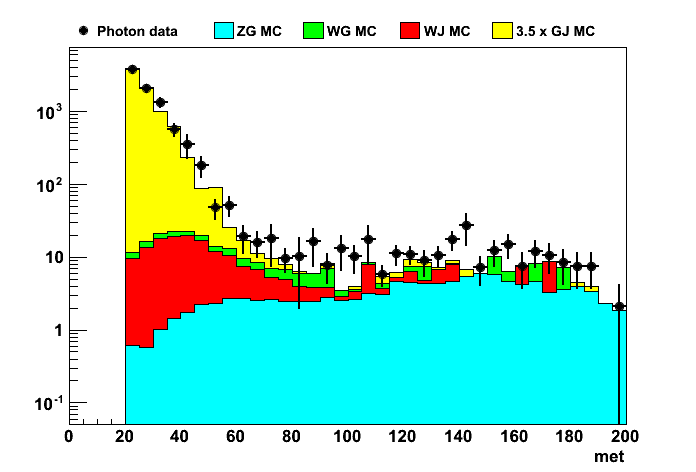
\includegraphics[width=.4\textwidth]{figures/met_0j.png}}\\
\subfigure[proj-trackMet in \dyll~ sample]{\label{subfig:pTrackMet_0j}
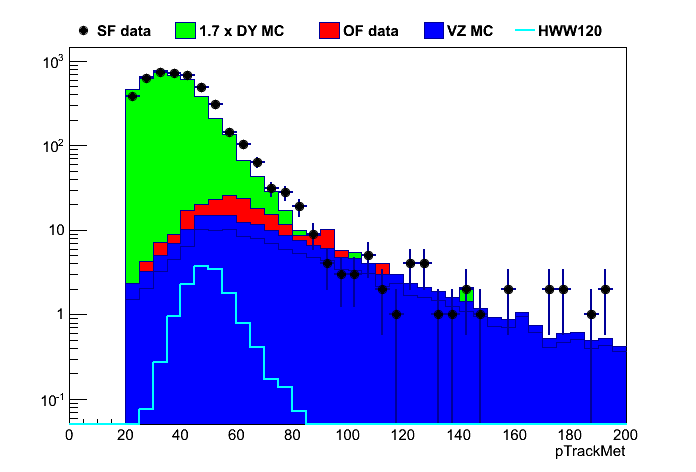
\includegraphics[width=.4\textwidth]{figures/pTrackMet_0j.png}}
\subfigure[trackMet in \gjets~ sample]{\label{subfig:trackMet_0j}
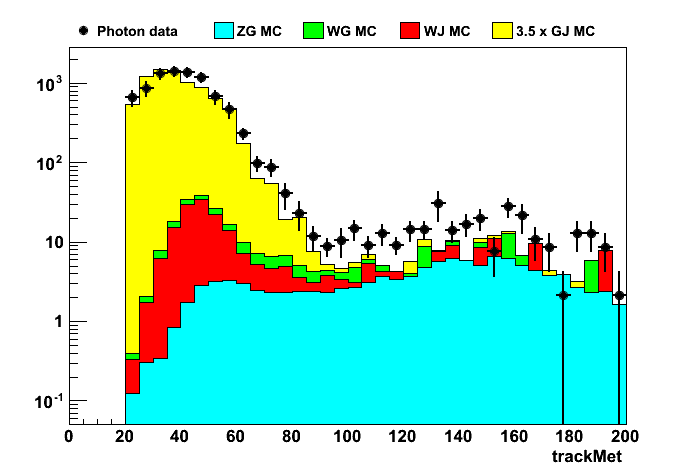
\includegraphics[width=.4\textwidth]{figures/trackMet_0j.png}}
\caption{\met in the 0-jet bin. 
For visualization purposes, the \gjets~ and \dyll~contributions from MC are scaled by a had-hoc scale factor to macth data in the bulk of the distribution.
In the \gjets~ sample, data is shown after re-weighting to the \dyll~$p_T$ distribution in MC events.}
\label{fig:met_0j}
\end{center}
\end{figure}
%%%%%%%%

%%%%%%%%
\begin{figure}[!hbtp]
\begin{center}
\subfigure[proj-pfMet in \dyll~ sample]{\label{subfig:pmet_1j}
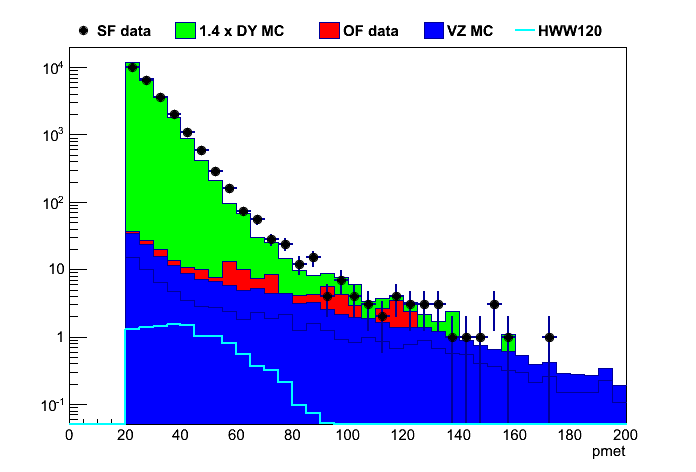
\includegraphics[width=.4\textwidth]{figures/pmet_1j.png}}
\subfigure[pfMet in \gjets~ sample]{\label{subfig:met_1j}
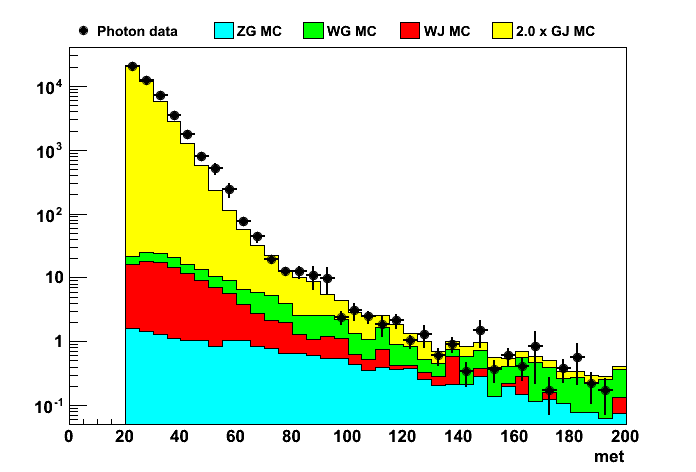
\includegraphics[width=.4\textwidth]{figures/met_1j.png}}\\
\subfigure[proj-trackMet in \dyll~ sample]{\label{subfig:pTrackMet_1j}
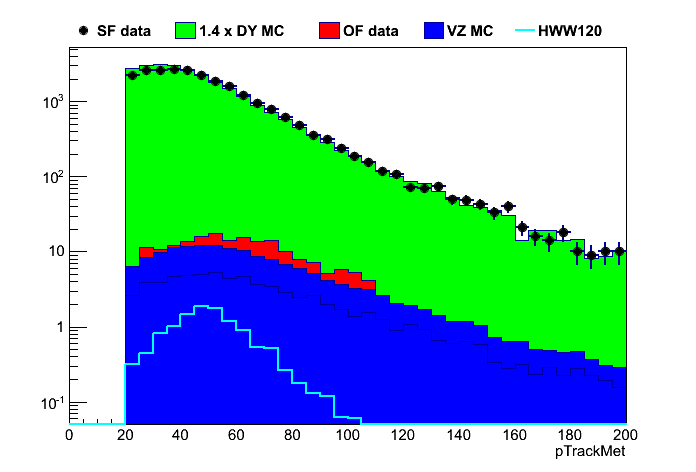
\includegraphics[width=.4\textwidth]{figures/pTrackMet_1j.png}}
\subfigure[trackMet in \gjets~ sample]{\label{subfig:trackMet_1j}
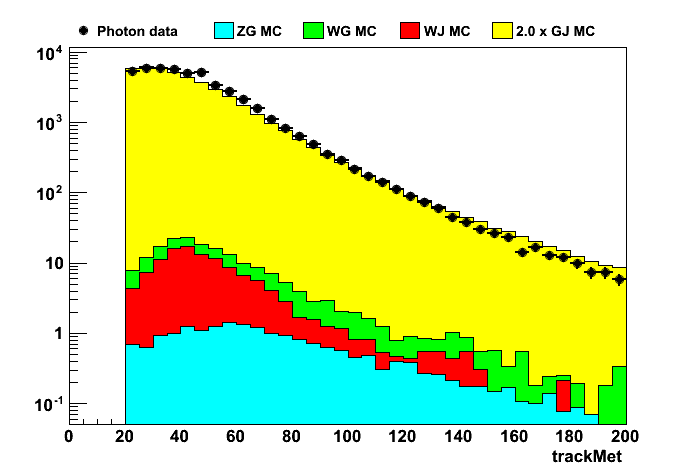
\includegraphics[width=.4\textwidth]{figures/trackMet_1j.png}}
\caption{\met in the 1-jet bin. 
For visualization purposes, the \gjets~ and \dyll~contributions from MC are scaled by a had-hoc scale factor to macth data in the bulk of the distribution.
In the \gjets~ sample, data is shown after re-weighting to the \dyll~$p_T$ distribution in MC events.}
\label{fig:met_1j}
\end{center}
\end{figure}
%%%%%%%%

%%%%%%%%
\begin{figure}[!hbtp]
\begin{center}
\subfigure[proj-pfMet in \dyll~ sample]{\label{subfig:pmet_2j}
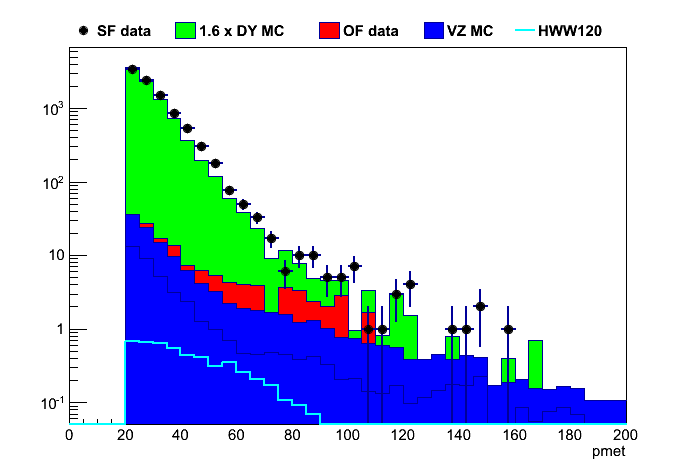
\includegraphics[width=.4\textwidth]{figures/pmet_2j.png}}
\subfigure[pfMet in \gjets~ sample]{\label{subfig:met_2j}
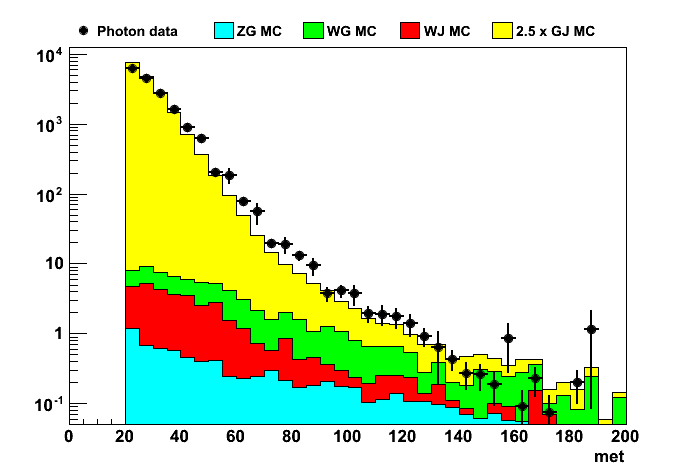
\includegraphics[width=.4\textwidth]{figures/met_2j.png}}\\
\subfigure[proj-trackMet in \dyll~ sample]{\label{subfig:pTrackMet_2j}
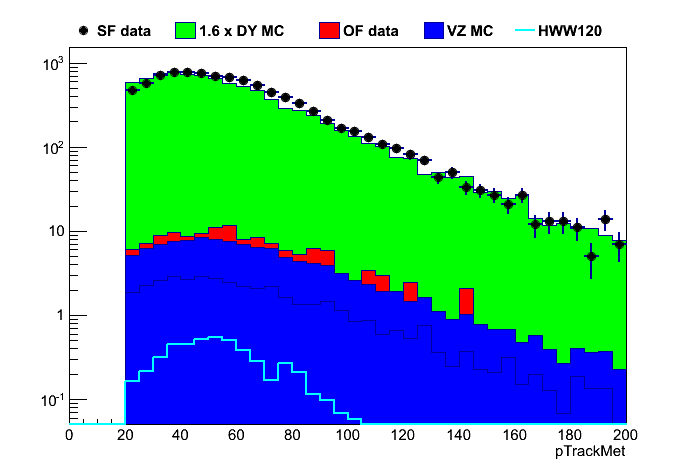
\includegraphics[width=.4\textwidth]{figures/pTrackMet_2j.png}}
\subfigure[trackMet in \gjets~ sample]{\label{subfig:trackMet_2j}
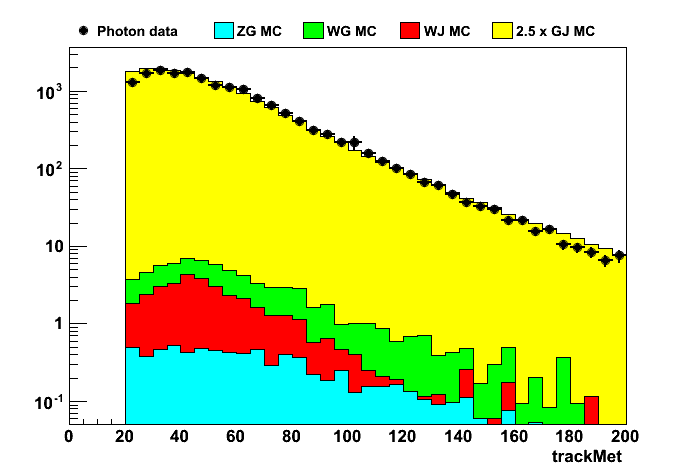
\includegraphics[width=.4\textwidth]{figures/trackMet_2j.png}}
\caption{\met in the 2-jet bin. 
For visualization purposes, the \gjets~ and \dyll~contributions from MC are scaled by a had-hoc scale factor to macth data in the bulk of the distribution.
In the \gjets~ sample, data is shown after re-weighting to the \dyll~$p_T$ distribution in MC events.}
\label{fig:met_2j}
\end{center}
\end{figure}
%%%%%%%%

\clearpage

\subsection{Evaluation of \zm}

For each jet bin, \zm~ is evaluated both on MC and data samples in bins of photon $p_T$.
In data, the expected backgrounds with non-fake \met~ are subtracted from the photon sample.
Results for WW level in  are shown in Figures~\ref{fig:zeta_MC} and~\ref{fig:zeta_mh0}.
These are the values used for the \hww~ BDT shape analysis.

In the cut based analysis, an additional narrow cut on the transverse Higgs mass is applied~\cite{ref:hwwsmurfs}, where the following definition of $m_T$ is used:
\begin{equation}
m_{T} = \sqrt{2\pt^{ll}\met(1-cos(\Delta\phi_{\ell\ell-\met}))}
\end{equation}
where $\Delta\phi_{\ell\ell-\met}$ is the angle between dilepton direction and \met\ in the transverse plane.
For example, in the \mHi=120 \GeVcc~ analysis the signal region requires 70$<$$m_T$$<$120 \GeVcc.
Given that \met\ and $m_T$ are correlated variables, the \zm\ value depends on the $m_T$ cut value; 
therefore, \zm\ is derived separately for each Higgs mass analysis applying the corresponding $m_T$ cut on the photon sample.

A few representative results for \zm~derived from data for Higgs level cut based analysis are shown in Figures~\ref{fig:zeta_mh120}-\ref{fig:zeta_mh160}.

%%%%%%%%
\begin{figure}[!hbtp]
\begin{center}
\subfigure[0-jet]{\label{subfig:zeta_MC_0j_minmet}
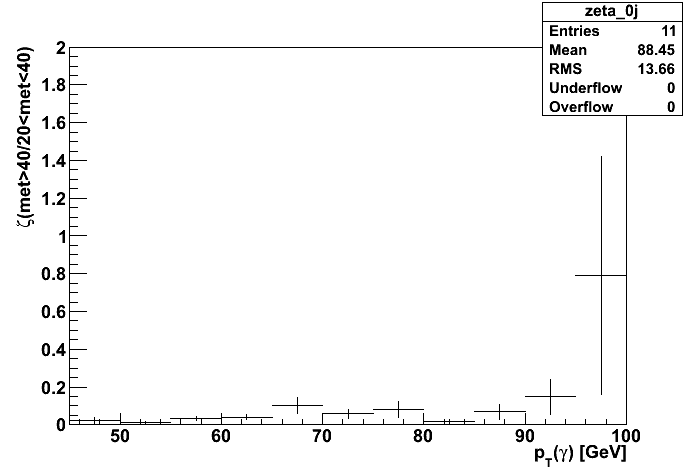
\includegraphics[width=.4\textwidth]{figures/zeta_MC_0j_minmet.png}}
\subfigure[1-jet]{\label{subfig:zeta_MC_1j_minmet}
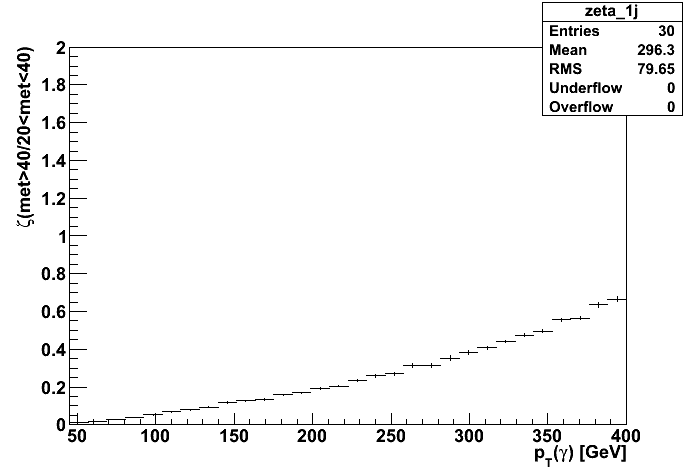
\includegraphics[width=.4\textwidth]{figures/zeta_MC_1j_minmet.png}}\\
\subfigure[2-jet]{\label{subfig:zeta_MC_2j_minmet}
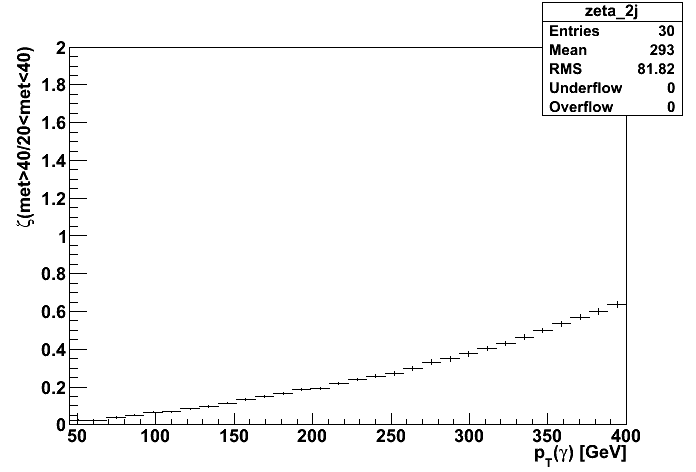
\includegraphics[width=.4\textwidth]{figures/zeta_MC_2j_minmet.png}}
\caption{\zm~in MC at \WW~level.}
\label{fig:zeta_MC}
\end{center}
\end{figure}
%%%%%%%%

%%%%%%%%
\begin{figure}[!hbtp]
\begin{center}
\subfigure[0-jet]{\label{subfig:zeta_mass0_0j_minmet}
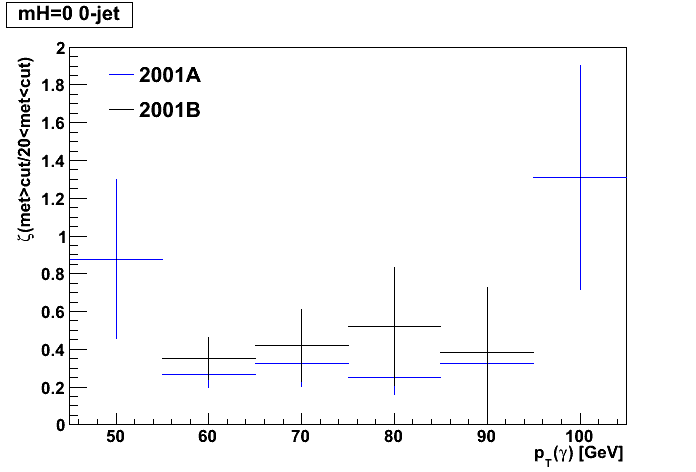
\includegraphics[width=.4\textwidth]{figures/zeta_mass0_0j_minmet.png}}
\subfigure[1-jet]{\label{subfig:zeta_mass0_1j_minmet}
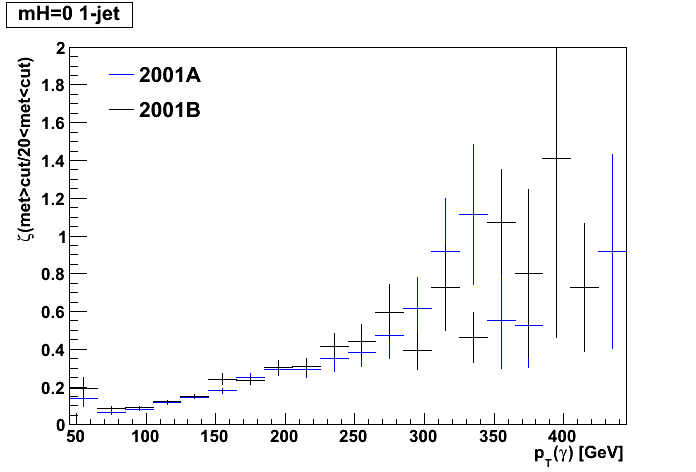
\includegraphics[width=.4\textwidth]{figures/zeta_mass0_1j_minmet.png}}\\
\subfigure[2-jet]{\label{subfig:zeta_mass0_2j_minmet}
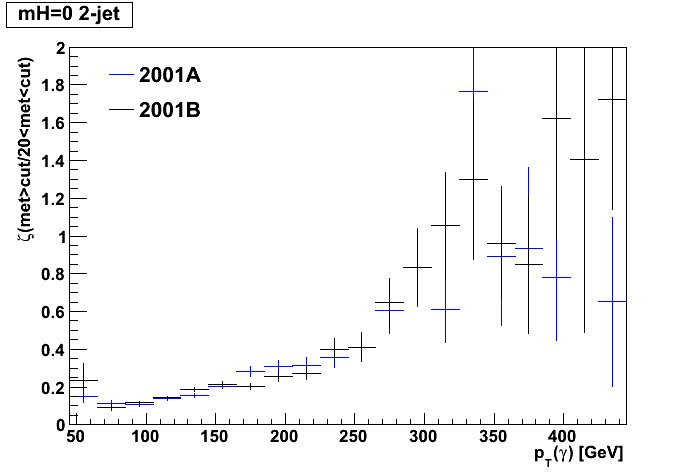
\includegraphics[width=.4\textwidth]{figures/zeta_mass0_2j_minmet.png}}
\caption{\zm~in data at \WW~level.}
\label{fig:zeta_mh0}
\end{center}
\end{figure}
%%%%%%%%

%%%%%%%%
\begin{figure}[!hbtp]
\begin{center}
\subfigure[0-jet]{\label{subfig:zeta_mass120_0j_minmet}
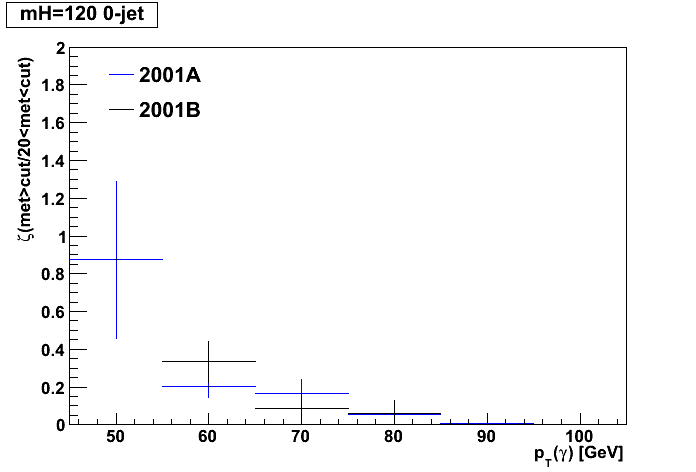
\includegraphics[width=.4\textwidth]{figures/zeta_mass120_0j_minmet.png}}
\subfigure[1-jet]{\label{subfig:zeta_mass120_1j_minmet}
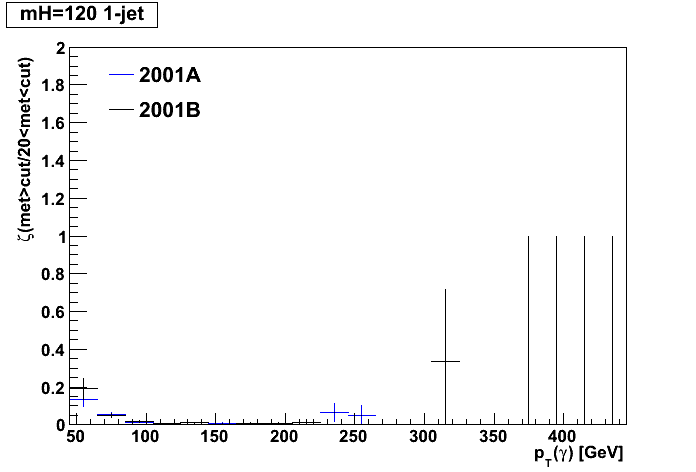
\includegraphics[width=.4\textwidth]{figures/zeta_mass120_1j_minmet.png}}\\
\subfigure[2-jet]{\label{subfig:zeta_mass120_2j_minmet}
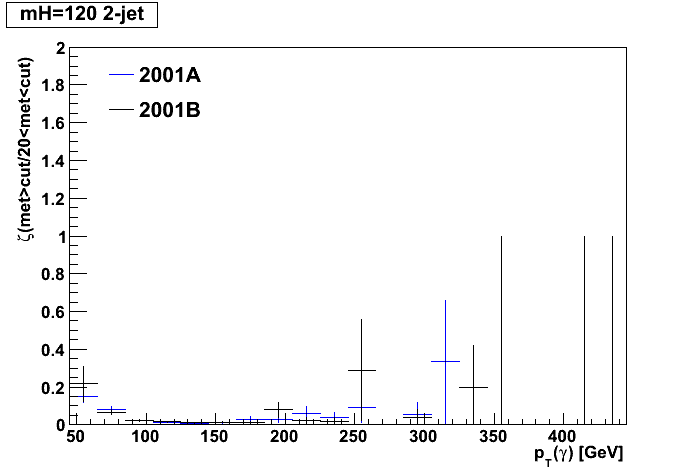
\includegraphics[width=.4\textwidth]{figures/zeta_mass120_2j_minmet.png}}
\caption{\zm~in data for \mHi=120 \GeVcc.}
\label{fig:zeta_mh120}
\end{center}
\end{figure}
%%%%%%%%

%%%%%%%%
\begin{figure}[!hbtp]
\begin{center}
\subfigure[0-jet]{\label{subfig:zeta_mass140_0j_minmet}
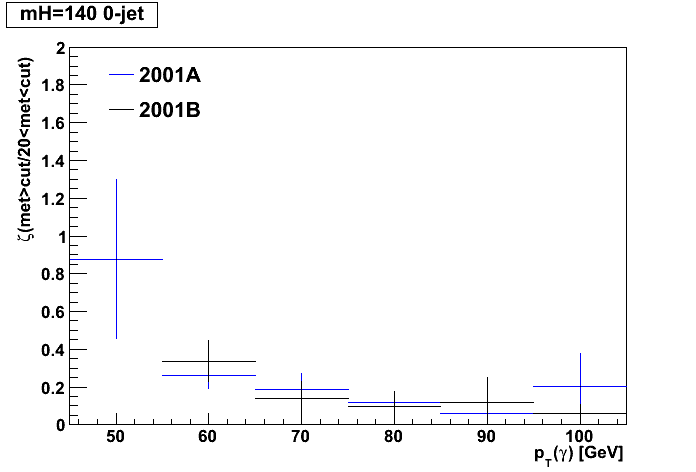
\includegraphics[width=.4\textwidth]{figures/zeta_mass140_0j_minmet.png}}
\subfigure[1-jet]{\label{subfig:zeta_mass140_1j_minmet}
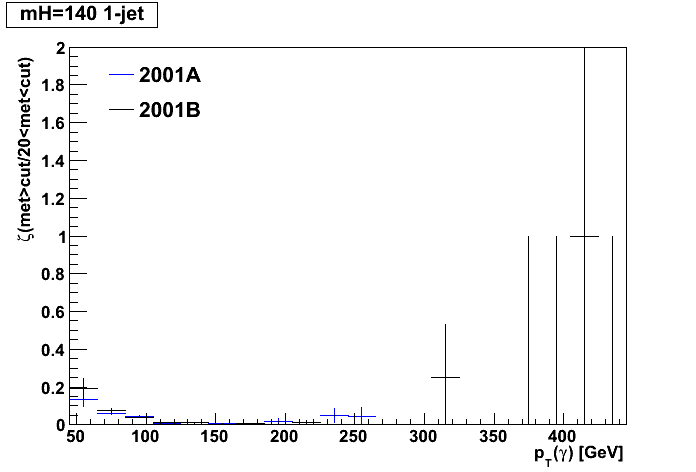
\includegraphics[width=.4\textwidth]{figures/zeta_mass140_1j_minmet.png}}\\
\subfigure[2-jet]{\label{subfig:zeta_mass140_2j_minmet}
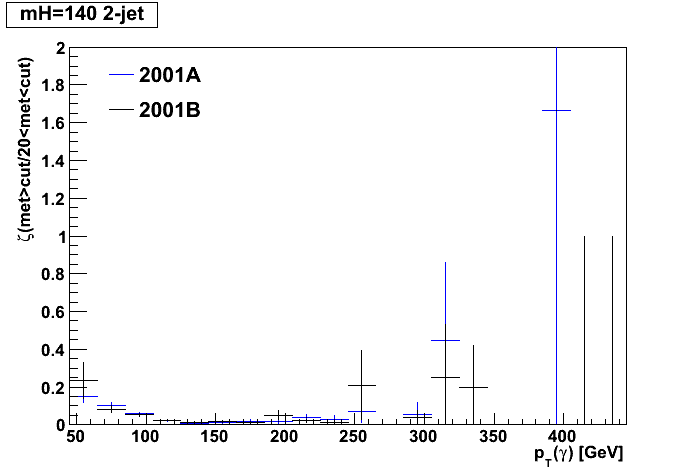
\includegraphics[width=.4\textwidth]{figures/zeta_mass140_2j_minmet.png}}
\caption{\zm~in data for \mHi=140 \GeVcc.}
\label{fig:zeta_mh140}
\end{center}
\end{figure}
%%%%%%%%

%%%%%%%%
\begin{figure}[!hbtp]
\begin{center}
\subfigure[0-jet]{\label{subfig:zeta_mass160_0j_minmet}
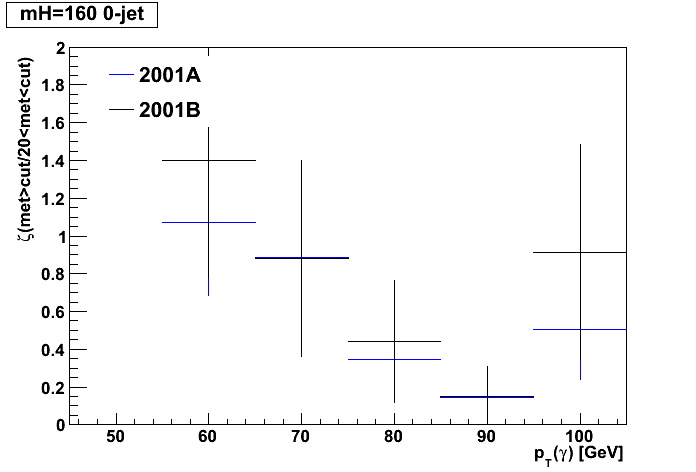
\includegraphics[width=.4\textwidth]{figures/zeta_mass160_0j_minmet.png}}
\subfigure[1-jet]{\label{subfig:zeta_mass160_1j_minmet}
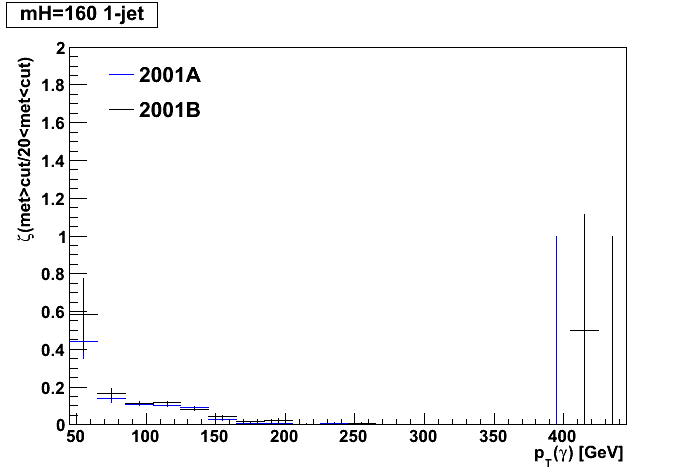
\includegraphics[width=.4\textwidth]{figures/zeta_mass160_1j_minmet.png}}\\
\subfigure[2-jet]{\label{subfig:zeta_mass160_2j_minmet}
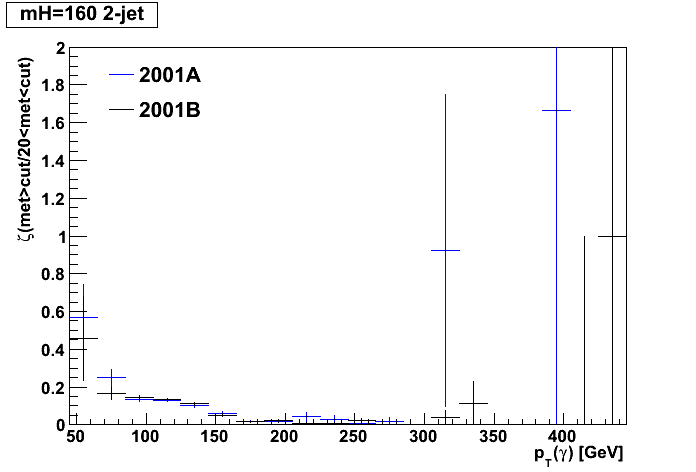
\includegraphics[width=.4\textwidth]{figures/zeta_mass160_2j_minmet.png}}
\caption{\zm~in data for \mHi=160 \GeVcc.}
\label{fig:zeta_mh160}
\end{center}
\end{figure}
%%%%%%%%

\clearpage
